\begin{frame}[ctb!]
  \frametitle{Mixed Cell Model Base Case II}
  \begin{figure}
\begin{minipage}[b]{0.45\linewidth}

  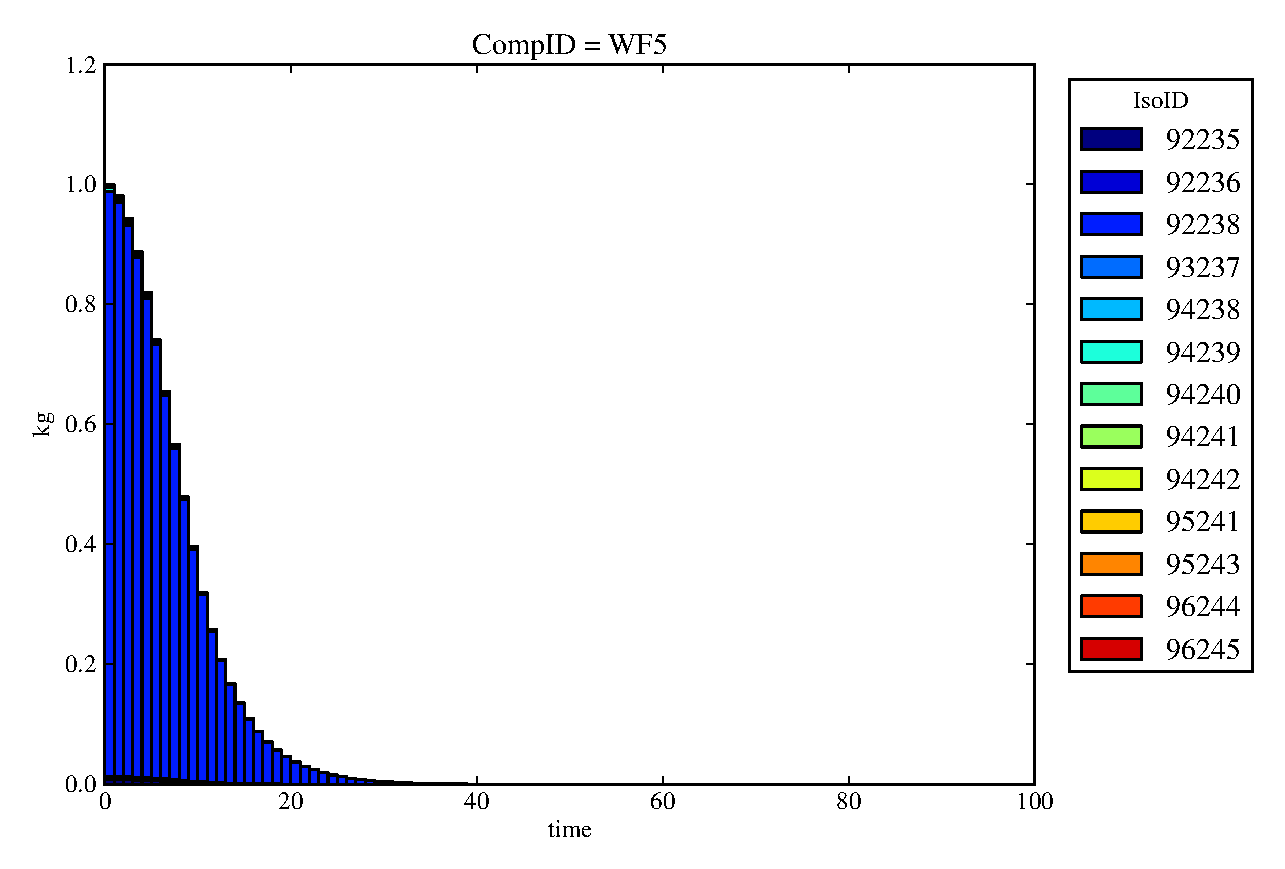
\includegraphics[width=0.8\textwidth]{./images/mcIII1.eps}
  \caption[MCI WF Contaminants.]{
    WF 5 releases material with degradation. 
    }
  \label{fig:mcIIIwf5}
  
  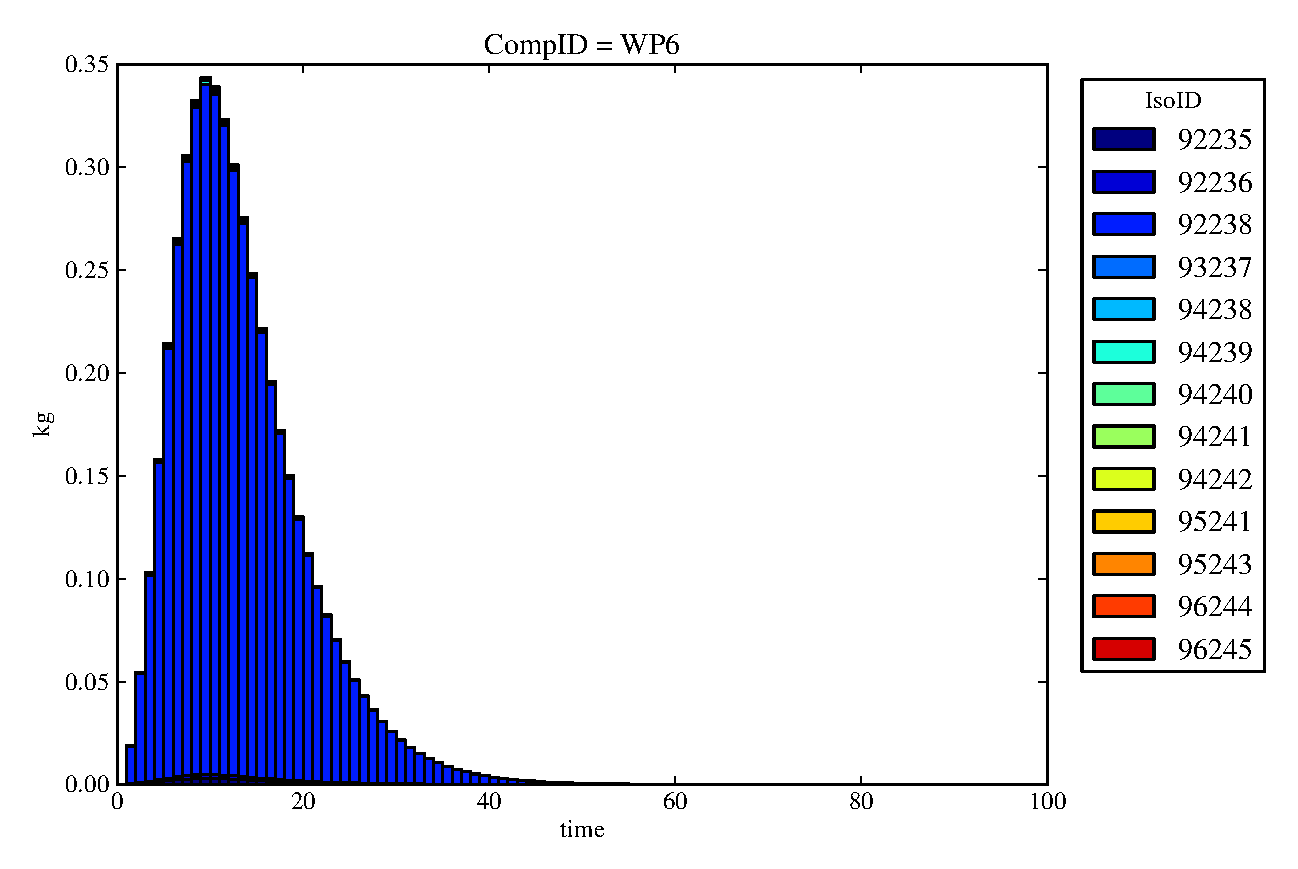
\includegraphics[width=0.8\textwidth]{./images/mcIII2.eps}
  \caption[Case MCI WP Contaminants.]{ 
    WP 6 receives and releases material. 
    }
  \label{fig:mcIIIwp6}

\end{minipage}
\hspace{0.05\linewidth}
\begin{minipage}[b]{0.45\linewidth}
  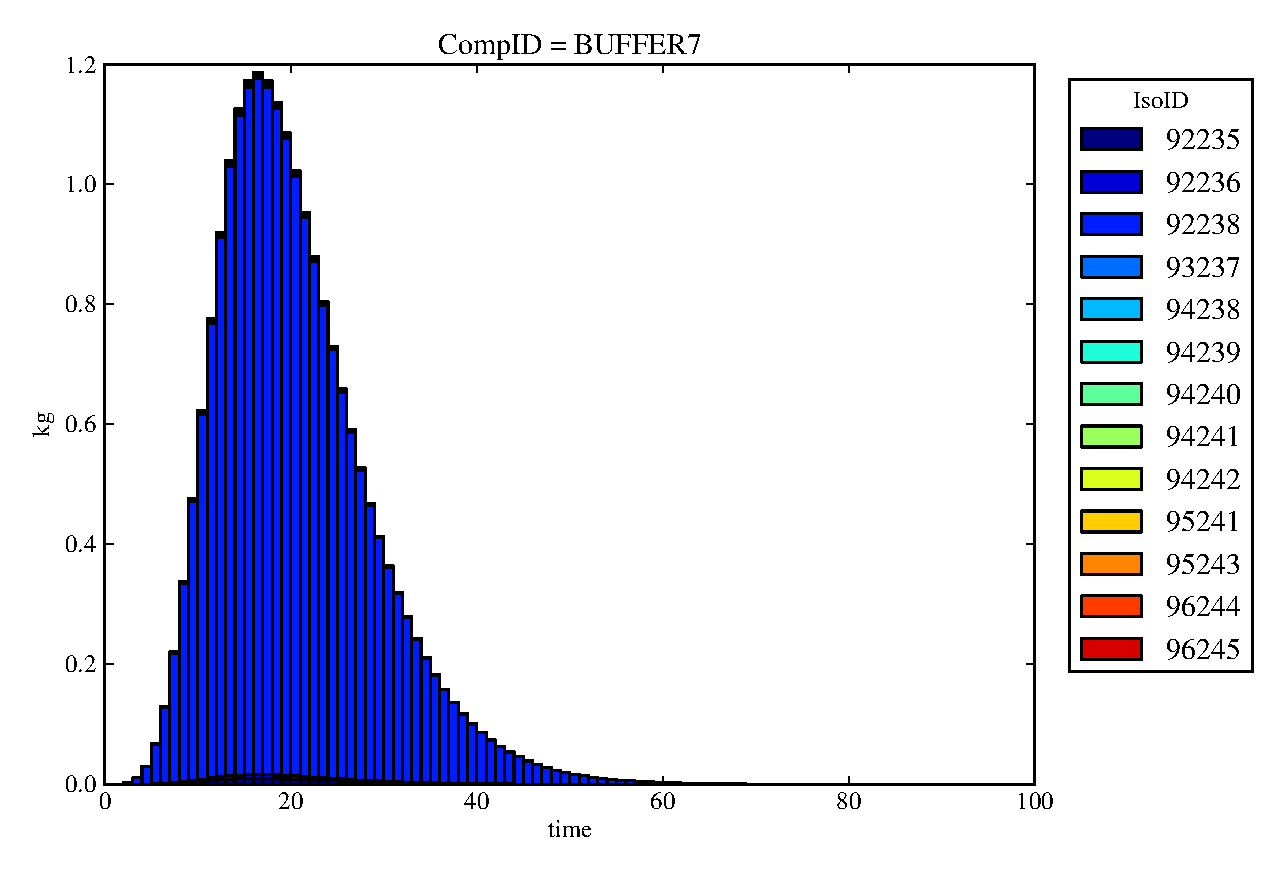
\includegraphics[width=0.8\textwidth]{./images/mcIII3.eps}
  \caption[Case MCI Buffer Contaminants]{
    Buffer 7, receives and releases material.
    }
  \label{fig:mcIIIbuff}

  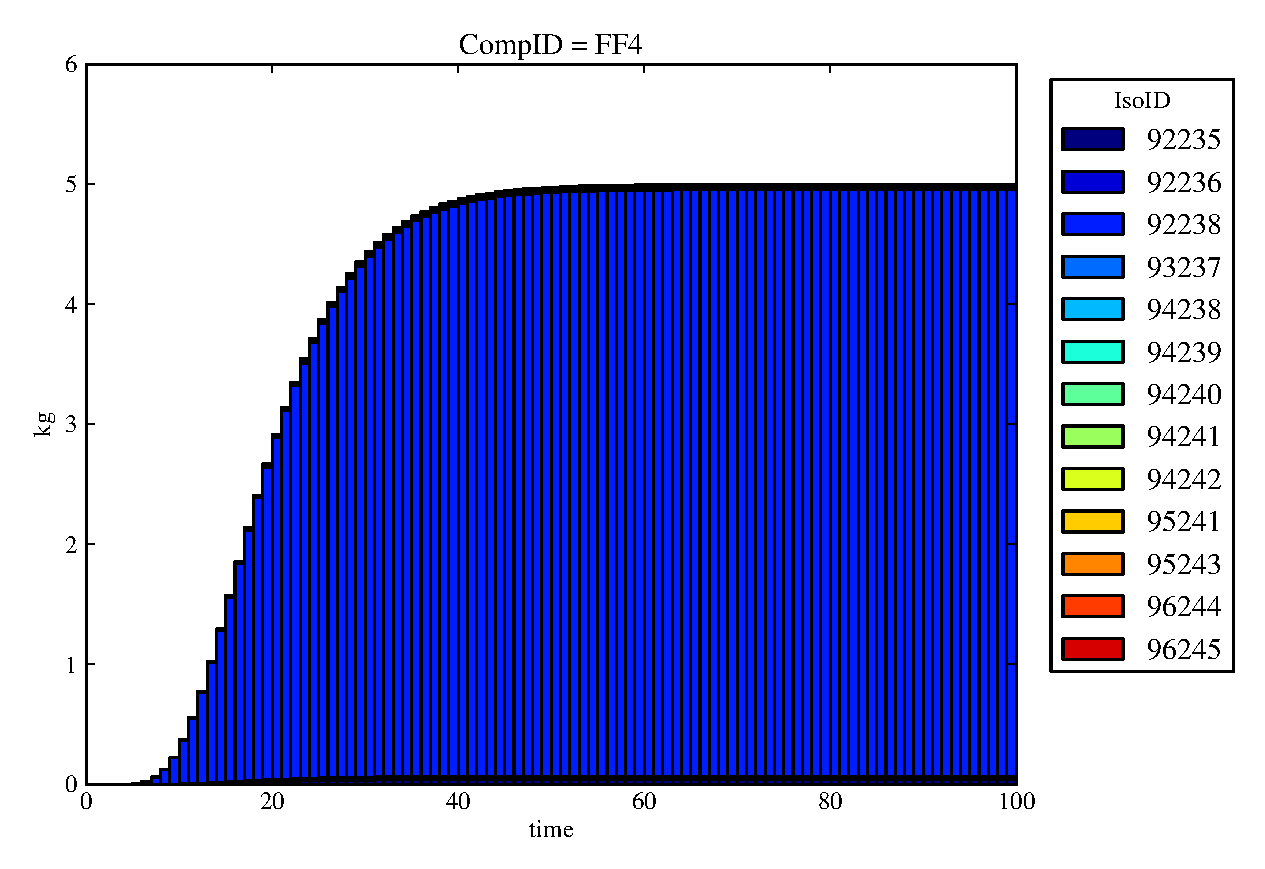
\includegraphics[width=0.8\textwidth]{./images/mcIII0.eps}
  \caption[Case MCI FF Contaminants.]{ 
    Far Field 4 acheives total containment.
    }
  \label{fig:mcII}


  \end{minipage}
\end{figure}

\end{frame}


\begin{frame}[ctb!]
  \frametitle{Mixed Cell Model Base Case II}
\begin{figure}[ht]
\centering
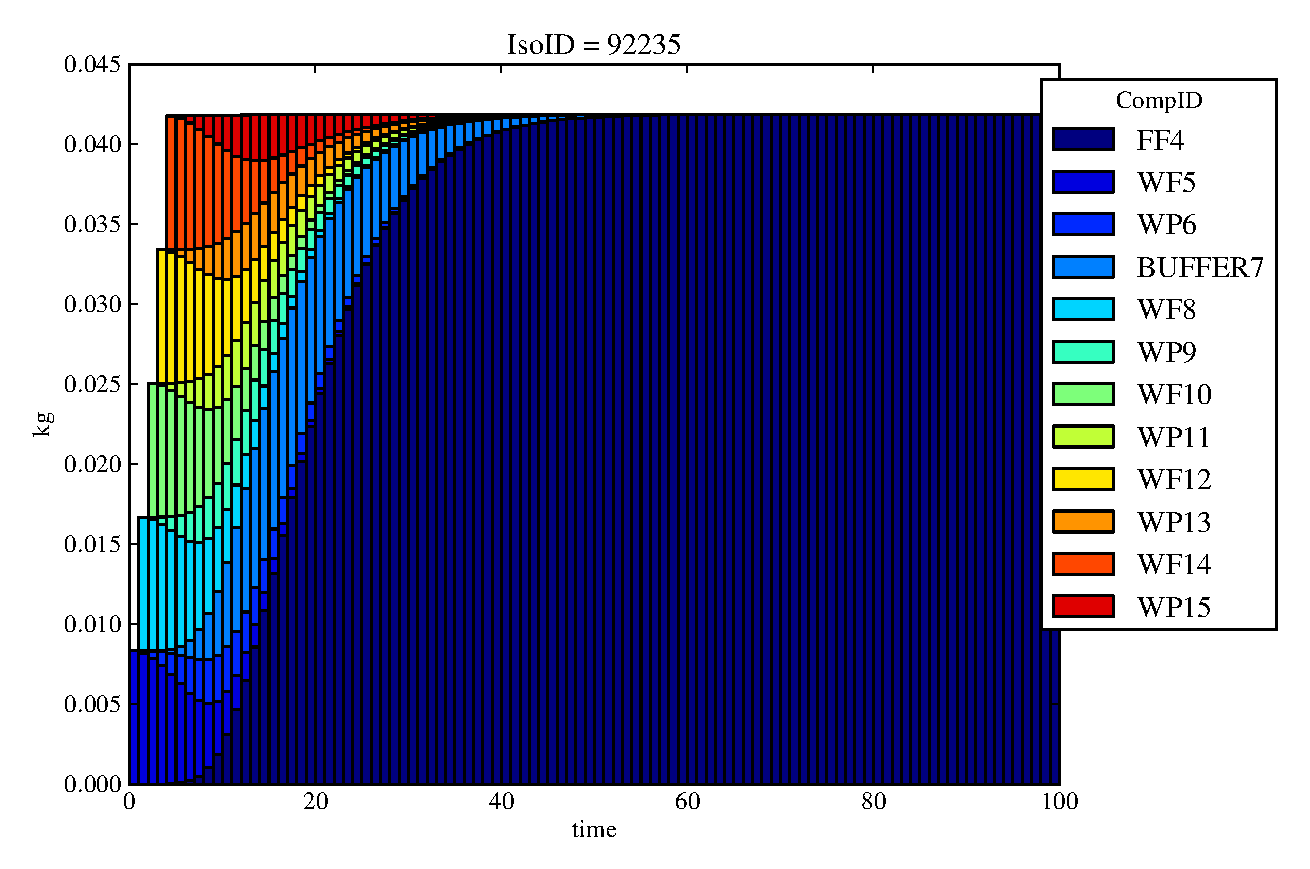
\includegraphics[width=0.8\textwidth]{./images/mcIII.eps}
\caption[$^{235}U$ residence. Mixed Cell Coupled Sorption and Solubility Limitation.]{
For the MCII case in which containment is affected by solubility limitation,
($F_{d}=0.1$, $S_{ref}=0.1kg/m^3$ for all components), $^{235}U$ travels more slowly
before permanent residence in the far field component.
}
\label{fig:mcIIIall}
\end{figure}
\end{frame}

